\documentclass[openany]{book}
\usepackage[utf8]{inputenc}
\usepackage{verbatim}
\usepackage[hypertexnames=false]{hyperref}
\usepackage{amstext} 
\usepackage{array}   
% \usepackage{nath}
\newcolumntype{C}{>{$}c<{$}} 


%%%%%%%%%%%%%%%%%%%%%%%

%%%%%%%%%%%%%%%%%%%%%%%
% HOLA PACO
% ESTE ES EL ARCHIVO DE LAS DEFINICIONES ESTRUCTURALES
% VERSION 1.1 NOMÁS
%
% AUTOR ORIGINAL:
% EDUARDO (CHITO) BELMONTE GUILLAMÓN
%
% ESTE ARCHIVO ES COMUNISTA, PUEDES COMPARTIRLO SI QUIERES
%%%%%%%%%%%%%%%%%%%%%%%

%----------------------------------
%     PAQUETICOS QUE SE USAN
%----------------------------------

%--------------------------
%    PARA USAR INKSCAPE
%---------------------------
\usepackage{import}
\usepackage{hyperref}
\usepackage{xifthen}
\usepackage{pdfpages}
\usepackage{transparent}

\newcommand{\incfig}[1]{%
    \def\svgwidth{\columnwidth}
    \import{./figures/}{#1.pdf_tex}
}

\newcommand{\custincfig}[2]{%
    \def\svgwidth{#1}
    \import{./figures/}{#2.pdf_tex}
}
\newcommand{\textnexttofig}[3]{
  \begin{minipage}[l]{0.45\textwidth}
    \custincfig{#1}{#2}
  \end{minipage}
  \begin{minipage}[l]{0.45\textwidth}
    #3
  \end{minipage}
}

%%%%%%%%% FIN DEL INKSCAPE

\usepackage{parskip} % Pa parrafos wapos
\setlength{\parindent}{0.5cm} % Pa la sangría
\usepackage{graphicx} % Pa meter las imágenes
\graphicspath{{Images/}} % La ruta a las imágenes

\usepackage{tikz} % Pa dibujar cosichuelas guapas

\usepackage[spanish]{babel} % PA QUE ESTÉ EN ESPAÑOL NOMÁS

\usepackage{enumitem} % Para personalizar las LISTAS YEAH

\setlist{nolistsep} % Pa que las listas estén junticas

\usepackage{booktabs} % Esta sirve para hacer tablas fancy con multicolumns y tal pero no tengo ni puta idea de usarla

\usepackage{xcolor} % PA DEFINIR LOS COLORINES
\definecolor{turquoise}{RGB}{21,103,112} % Es un turquesica así formal
\definecolor{violet}{RGB}{ 110, 6, 187 } % Color maricón

%-------------------------------------------------
%     MÁRGENES
%-------------------------------------------------

\usepackage{geometry}
\geometry{
    top=3cm,
    bottom=3cm,
    left=3cm,
    right=3cm,
    headheight=14pt,
	footskip=1.4cm,
	headsep=10pt,
}

\usepackage{avant} % Esto es una fuente para encabezados

%\usepackage{mathptmx} % Usar simbolitos matemáticos chulos

\usepackage{microtype} % Para fuentes de maricones

\usepackage[utf8]{inputenc} % Pa los acentos

\usepackage[T1]{fontenc}

%-------------------------------------------------
% Bibliografía e índice
%-------------------------------------------------

\usepackage{makeidx} % Pa hacer un índice
\makeindex

\usepackage{titletoc}   % Para manipular la tabla de contenidos

\contentsmargin{0cm}    % Para eliminar el margen por defecto

\usepackage{titlesec} % Pa cambiar los titulos skere

\titleformat
{\chapter} % command
[display] % shape
{\centering\bfseries\Huge\normalfont} % format
{\color{turquoise}  {\normalsize\MakeUppercase{Capítulo} \thechapter }} % label
{-0.5cm} % sep
{
    \color{turquoise}
    \rule{\textwidth}{3pt}
    \vspace{1ex}
    \centering
    \setcounter{ex}{0}
    \setcounter{dummy}{0}
} % before-code
[
\vspace{-0.5cm}%
\rule{\textwidth}{3pt}
] % after-code


\titleformat{\part}
[display]
{\centering\bfseries\Huge\normalfont}
{\color{turquoise} {\normalsize \MakeUppercase{Asignatura}}}
{0pt}
{\color{turquoise}
\vspace{-0.6cm}
\rule{\textwidth}{3pt}
\vspace{1ex}
\setcounter{chapter}{0}
\setcounter{section}{0}
\setcounter{dummy}{0}
\centering
}


\titleformat{\section}
{\normalfont\Large\bfseries}{\color{turquoise}\thesection\ - }{0.5em}{}

\usepackage{fancyhdr}   % Necesario para el encabezado y el pie de página

\pagestyle{fancy}   %Para modificar los encabezados
\fancyhf{}          %Para eliminar los encabezados y pies de página por defecto.
\fancyhead[LE,RO]{\sffamily\normalsize\thepage}
\fancyfoot[C]{Ampliación de Probabilidad}
%HACER

\usepackage{amsmath,amsfonts,amssymb,amsthm,cancel} % PARA LAS MATES

%   LINEA 199, HACER CAPULLADAS

\newtheoremstyle{turquoisebox}
{0pt} %Espacio encima
{0pt} %Espacio abajo
{\normalfont} % Fuente del cuerpo
{} % Cantidad de identado
{\small\ssfamily\color{turquoise}} % Fuente en la que pone "TEOREMA"
{:} % Puntuación tras el teorema
{0.25em} %Espacio tras el teorema
{\thmname{#1}\thmnumber{#2}} %No sé si esto funciona


\newcounter{dummy}
\newcounter{ex}
\newtheorem{teoremote}[dummy]{\color{turquoise}Teorema}
\newtheorem{propositiont}{\color{turquoise}Proposición}[section]
\newtheorem{lemmat}{\color{turquoise}Lema}[section]
\newtheorem{definitionT}{\color{turquoise}Definición}[section]
\newtheorem{exerciseT}[ex]{Ejercicio}
\newtheorem{examplote}[ex]{\color{turquoise}Ejemplo}
\newtheorem{methodT}[dummy]{\color{turquoise}Método}


\RequirePackage[framemethod=default]{mdframed} % Required for creating the theorem, definition, exercise and corollary boxes

%Caja de teoremas

\newmdenv[skipabove=7pt,
skipbelow=7pt,
backgroundcolor=black!5,
linecolor=turquoise,
innerleftmargin=5pt,
innerrightmargin=5pt,
innertopmargin=5pt,
leftmargin=0cm,
rightmargin=0cm,
linewidth=3pt,
innerbottommargin=5pt]{tBox}

\newmdenv[skipabove=7pt,
skipbelow=7pt,
backgroundcolor=black!5,
linecolor=turquoise,
innerleftmargin=5pt,
innerrightmargin=5pt,
innertopmargin=5pt,
leftmargin=0cm,
rightmargin=0cm,
linewidth=1pt,
innerbottommargin=5pt]{pBox}

\newmdenv[skipabove=7pt,
skipbelow=7pt,
backgroundcolor=violet!7,
linecolor=turquoise,
innerleftmargin=5pt,
innerrightmargin=5pt,
innertopmargin=5pt,
leftmargin=0cm,
rightmargin=0cm,
rightline=false,
topline=false,
bottomline=false,
linewidth=4pt,
innerbottommargin=5pt]{mBox}

\newmdenv[skipabove=7pt,
skipbelow=7pt,
rightline=false,
leftline=true,
topline=false,
bottomline=false,
linecolor=turquoise,
innerleftmargin=5pt,
innerrightmargin=5pt,
innertopmargin=0pt,
leftmargin=0cm,
rightmargin=0cm,
linewidth=4pt,
innerbottommargin=0pt]{dBox}

\newmdenv[skipabove=7pt,
skipbelow=7pt,
rightline=false,
leftline=true,
topline=false,
bottomline=false,
backgroundcolor=black!3,
linecolor=turquoise!50,
innerleftmargin=5pt,
innerrightmargin=5pt,
innertopmargin=0pt,
innerbottommargin=5pt,
leftmargin=0cm,
rightmargin=0cm,
linewidth=4pt]{eBox}

\newmdenv[skipabove=7pt,
skipbelow=7pt,
leftline=true,
topline=false,
rightline=false,
bottomline=false,
backgroundcolor=cyan!5,
linecolor=turquoise,
innerleftmargin=5pt,
innerrightmargin=5pt,
innertopmargin=0pt,
innerbottommargin=5pt,
leftmargin=0cm,
rightmargin=0cm,
linewidth=4pt]{exBox}

\newenvironment{theorem}{\begin{tBox}\begin{teoremote}}{\end{teoremote}\end{tBox}}
\newenvironment{proposition}{\begin{pBox}\begin{propositiont}}{\end{propositiont}\end{pBox}}
\newenvironment{lemma}{\begin{pBox}\begin{lemmat}}{\end{lemmat}\end{pBox}}
\newenvironment{method}{\begin{mBox}\begin{methodT}}{\end{methodT}\end{mBox}}
\newenvironment{definition}{\begin{dBox}\begin{definitionT}}{\end{definitionT}\end{dBox}}
\newenvironment{exercise}{\begin{eBox}\begin{exerciseT}}{\hfill{\color{black}}\end{exerciseT}\end{eBox}}
\newenvironment{example}{\begin{exBox}\begin{examplote}}{\end{examplote}\end{exBox}}
\newenvironment{demonstration}{\begin{flushright}
      \color{turquoise} \textbf{Demostración}
\end{flushright}
}{\begin{flushright}
  $\square$
\end{flushright}}

\usepackage{geometry}
\geometry{
    top=3cm,
    bottom=3cm,
    left=3cm,
    right=3cm,
    headheight=14pt, 
    footskip=1.4cm,
    headsep=10pt,
}
\usepackage{graphicx}
\title{Ejercicios de Ampliación de Probabilidad}
\author{Paco Mora Caselles}
\date{\today}

\begin{document}

\maketitle

\chapter{Relación 1}
\begin{exercise}
    $$  C = \{(x,y) \in \mathbb{R} ^2 \ :\ 0<x<1,\ 0<y<1,\ y < (1-x)^2\} $$

    \begin{center}
        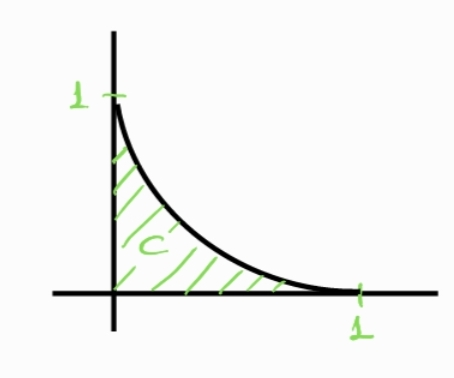
\includegraphics[scale=0.5]{1-1.jpg}
    \end{center}

    Dejamos por ahora $ f $ en función de $ k $, más tarde calculamos su valor:

    $$ f(x,y) = \left\{
    \begin{array}{lr}
        k & (x,y) \in C\\
        0 & (x,y) \not \in C   
    \end{array}
    \right. $$

    Para $ x \in (0,1) $:
    $$ f_{1}(x) = \int\limits_{}^{}f(x,y) dy = \int\limits_{0}^{(1-x)^2}k dy = k(1-x)^2 $$

    Entonces tenemos:

    $$ f_{1}(x) = \left\{
    \begin{array}{lr}
        k(1-x)^2 & x \in (0,1)\\
        0 & x \not \in (0,1)
    \end{array}
    \right. $$

    Pasamos ahora a $ f_{2}(y) $, cuando $ y \in (0,1) $:
    $$ f_{2}(y) = \int\limits_{}^{}f(x,y)dx = \int\limits_{0}^{1-y^{1/2}} = k (1-y)^{1/2} $$

    $$ f_{2}(y) = \left\{
    \begin{array}{lr}
        k(1-\sqrt{y}) & y \in (0,1) \\
        0 & y \not \in (0,1)
    \end{array}
    \right. $$

    Calculamos ahora $ E(X^{n}(1-X)^{m}) $ usamos $ f_{1}(x) $:
    $$ E(X^{n}(1-X)^{m}) = \int\limits_{}^{}x^{n}(1-x)^{m}f_{1}(x)dx = \int\limits_{0}^{1} x^{n}(1-x)^{m} k (1-x)^2 dx = k \int\limits_{0}^{1}x^{n}(1-x)^{m+2} =$$
    $$ =  kB(n+1,m+3) = k \dfrac{\Gamma(n+1)\Gamma(m+3)}{\Gamma(n+m+4)} = k \dfrac{n!(m+2)!}{(n+m+3)!} $$
    
    Los momentos de orden $ n $ respecto del origen, la esperanza y la varianza de $ X $ las podemos calcular con esta expresión. Para los primeros casos tomamos $ m=0 $ y para la varianza podemos usar que $ Var(X) = E(X^2)-E(X)^2 $

    $$ k = 3 \hspace{10mm} E(X) = \dfrac{1}{4}\hspace{10mm} E(X^2) = \dfrac{1}{10} \hspace{10mm} Var(X) = \dfrac{3}{80} $$
    
    Calculamos $ f_{2|1}(y|x) $, si $ x \in (0,1) $:
    $$ f_{2|1}(y|x) = \dfrac{f(x,y)}{f_{1}(x)} = \left\{
    \begin{array}{lr}
        \dfrac{3}{3(1-x)^2} = \dfrac{1}{(1-x)^2} & y \in (0,(1-x)^2)\\
        0 & y \not \in (0,(1-x)^2)
    \end{array}
    \right. $$

    Podemos calcular ahora $ f_{2|1}(y|x=1/2) $:
    $$ f_{2|1}(y|1/2) = \left\{
    \begin{array}{lr}
        4 & y \in (0,\dfrac{1}{4}) \\\\
        0 & y \not \in (0,\dfrac{1}{4})
    \end{array}
    \right. $$

    Para calcular $ F\left(\dfrac{1}{4},\dfrac{9}{16}\right) $ nos apoyamos en la figura para saber que basta con calcular el área del rectángulo y multiplicar por $ k $:
    
    \begin{center}
        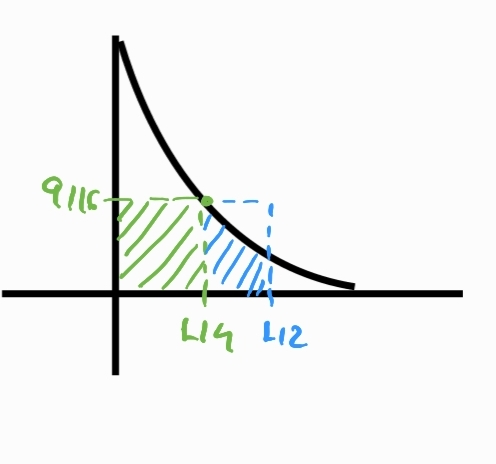
\includegraphics[scale=0.4]{1-1-2.jpg}
    \end{center}
    

    $$ F\left(\dfrac{1}{4},\dfrac{9}{16}\right) = 3 \dfrac{1}{4}\cdot \dfrac{9}{16} = \dfrac{3^3}{2^{6}}$$

    Para $ F\left(\dfrac{1}{2},\dfrac{9}{16}\right) = F\left(\dfrac{1}{4},\dfrac{9}{16}\right)+3\cdot Area\ T $, siendo $ T $ la intersección con $ C $. Sabemos entonces que:
    $$ \int\limits_{1/4}^{1/2}(1-x)^2dx = \int\limits_{1/4}^{1/2}(x^2-2x+1)dx = \dfrac{x^3}{3}-x^2+x \Biggr|_{1/4}^{1/2} = \dfrac{19}{2^{6}3} $$
    $$ F\left(\dfrac{1}{2},\dfrac{9}{16}\right) = \dfrac{3^3}{2^{6}} + 3 \dfrac{19}{2 ^{6}3} = \dfrac{23}{32} $$

    Tenemos que calcular ahora la recta de regresión de $ Y $ respecto de $ X $:
    $$ y - \mu_{y} = \dfrac{\sigma _{xy}}{\sigma_{x}^2}(x-\mu_{x}) $$
    $$ \mu_{y} = E(Y) = \int\limits_{0}^{1} y 3(1-y^{1/2})dy = 3 \int\limits_{0}^{1}(y-y^{3/2}) = \dfrac{3}{10} $$
    $$ E(XY) = \int\limits_{0}^{1} \int\limits_{0}^{(1-x)^2} 3xy dy dx = 3 \int\limits_{0}^{1} x \left[\dfrac{y^2}{2}\right]_{0} ^{(1-x)^2} d = \dfrac{3}{2} \int\limits_{0}^{1}x(1-x)^{4}dx = $$
    $$ = B(2,5) = \dfrac{3}{2} \dfrac{\Gamma(2)\Gamma(5)}{\Gamma(7)}= \dfrac{3}{2} \dfrac{1!4!}{6!} = \dfrac{1}{20} $$
    Recordemos que $ \mu_{X} = E(X) = \dfrac{1}{4} $, entonces:
    $$ \sigma_{XY}Cov(X,Y) = \dfrac{1}{2^2\cdot 5} -\dfrac{1}{2^2}\cdot \dfrac{3}{2\cdot 5} = \dfrac{2-3}{2^3\cdot 5} = -\dfrac{1}{2^3\cdot 5}$$

    Podemos expresar ya la recta de regresión (recordando que $ \sigma_{X}  = \dfrac{3}{80}$):
    $$ y-\dfrac{3}{10} = \dfrac{-1/(5\cdot 2^3)}{3/(2^{4}\cdot 5)}(x-\dfrac{1}{4}) $$
    $$ y = -\dfrac{2}{3}x+\dfrac{7}{15} $$

    Calculamos ahora $ E(Y|X=x) = m_{2|1}(x) $:
    $$ E(Y|X=x) = \int\limits_{}^{}y f_{2|1}(y|x)dy = \int\limits_{0}^{(1-x)^2}y \dfrac{1}{(1-x)^2}dy = $$
    $$ =\dfrac{1}{(1-x)^2} \dfrac{y^2}{2} \Biggr|_{0}^{(1-x)^2} = \dfrac{1}{(1-x)^2} \dfrac{(1-x)^{4}}{2} = \dfrac{(1-x)^2}{2} $$


\end{exercise}


\begin{exercise}
    $$ E(X) = 2,\ Var(X) = 3\ X\ \text{simétrica} $$
    
    $$ \alpha_{3} = E(X^3) = E((X-2+2)^3) = E((X-2)^3+3(X-2)^22+3(X-2)2^2+2^3) = $$
    $$= E((X-2)^3)+6E((X-2)^2) +12 E(X-2)+E(2^3) = 0 + 6 Var(X)+0+2^3 = 6\cdot 3+8 = 26$$
\end{exercise}


\begin{exercise}
    $  $\\
    El número de de posibilidades totales es claramente $ \binom{N}{n} $, la distribución de probabilidad es entonces:

    $$ P(X_1=r_1,X_2=r_2,X_3=r_3) = \dfrac{\binom{n_1}{r_1}\binom{n_2}{r_2}\binom{n_3}{r_3}}{\binom{N}{n}} $$
    Claramente necesitamos $ n\leq N,\ r_1+r_2+r_3=n $

    Calculamos ahora $ \alpha_{(3)} $:
    $$ E(X_1 ^{(3)}) = E(X_1(X_1-1)(X_1-2)) = \sum\limits_{r_1+r_2+r_3=n}^{}r_1(r_1-1)(r_1-2)\dfrac{\binom{n_1}{r_1}\binom{n_2}{r_2}\binom{n_3}{r_3}}{\binom{N}{n}} $$

    Nos fijamos que:

    $$r_1(r_1-1)(r_1-2)  \binom{N_1}{r_1} = r_1(r_1-1)(r_1-2) \dfrac{N_1 ^{(r_1)}}{r_1(r_1-1)(r_1-2)\cdots 2\cdot 1} = $$
    $$ =\dfrac{N_1 ^{(r_1)}}{(r_1-3)!} = N_1(N_1-1)(N_1-2) \dfrac{(N_1-3) ^{(r_1-3)}}{(r_1-3)!}  = N_1(N_1-1)(N_1-2)\binom{N_1-3}{r_1-3}$$

    Entonces volviendo a la igualdad anterior:
    $$ P(X_1=r_1) = \sum\limits_{r_1+r_2+r_3=n}^{}N_1(N_1-1)(N_1-2) \dfrac{\binom{N_1-3}{r_1-3}\binom{N_2}{r_2}\binom{N_3}{r_3}}{\binom{N}{n}} =  $$
    $$ N_1(N_1-1)(N_1-2)\sum\limits_{r_1+r_2+r_3=n}^{} \dfrac{\binom{N_1-3}{r_1-3}\binom{N_2}{r_2}\binom{N_3}{r_3}}{\binom{N}{n}} = N_1(N_1-1)(N_1-2) \dfrac{\binom{N-3}{n-3}}{\binom{N}{n}} =$$
    $$ = N_1(N_1-1)(N_2-2) \dfrac{(N-3) ^{(n-3)}n!}{(n-3)!N ^{(n)}} = \dfrac{N_1 ^{(3)}n ^{(3)}}{N ^{(3)}} $$
\end{exercise}


\begin{exercise}
    $  $
    \begin{flushright}
        \textbf{Aparado a)}
    \end{flushright}

    Observemos primero que no hay dos pares de la forma $ (a,b),\ (a,c) $ de forma que ambos tengan probabilidad no nula. Igual forma, no hay pares $ (b,a),\ (c,a) $ tales que se tomen ambos valores con probabilidad no nula. Por tanto, para ver la distribución marginal de $ X $ podemos omitir los valores que toma $ Y $:
    $$ P(X=0) = P(X=1) = P(X=2) = \dfrac{1}{3} $$

    De forma análoga para la v.a. $ Y $: 
    $$ P(Y=1) = P(Y=2) = P(Y=3) = \dfrac{1}{3} $$

    Las esperanzas entonces de estas vvaa son:
    $$ E(X) = (0+1+2)\cdot \dfrac{1}{3} = 1 $$
    $$ E(Y) = (1+2+3)\cdot \dfrac{1}{3} = 2 $$

    Hacemos también los cálculos necesarios para hacer la recta de regresión:
    $$ E(XY) = (0\cdot 1+1\cdot 2+2\cdot 3) \dfrac{1}{3} = \dfrac{8}{3} $$
    $$ Cov(X,Y) = E(XY) - E(X)E(Y) = \dfrac{8}{3}*2 =\dfrac{2}{3} $$
    $$ E(X^2) = (0+1+4)\dfrac{1}{3} = \dfrac{5}{3} $$
    $$ Var(X) = E(X^2)-E(X)^2 = \dfrac{5}{3}-1 = \dfrac{2}{3} $$

    La recta de regresión de $ Y $ sobre $ X $ es entonces:
    $$ y-2 = \dfrac{\dfrac{2}{3}}{\dfrac{2}{3}}(x-1) \implies y -2 = x-1 \implies y = x+1 $$

    Calculamos ahora el coeficiente de correlación para poder ver $ Var(Y-X^{*}) $:
    $$ \rho = \dfrac{\sigma_{XY}}{\sigma_{X}\sigma_{Y}} = \dfrac{\dfrac{2}{3}}{\sqrt{\dfrac{2}{3}}\sqrt{\dfrac{2}{3}}} = 1 $$

    Este valor de $ \rho $ nos indica que $ X $ y $ Y $ son dependientes linealmente. Calculamos ahora $ Var(Y-X^*) $

    $$ Var(Y-X^*) = \sigma_{Y}^2(1-\rho ^2) = 0 $$

    \begin{flushright}
        \textbf{Aparado b)}
    \end{flushright}

    Para calcular las $ vvaa $ marginales solo tenemos que sumar los elementos de la misma fila o columna. Por ejemplo:

    $$ P(X=0) = \dfrac{1}{3}+\dfrac{1}{6}+\dfrac{1}{9} = \dfrac{11}{18} $$

    Obtenemos así:
    $$ P(X=0) = \dfrac{11}{18} \hspace{5mm} P(X=1) = \dfrac{5}{18} \hspace{5mm} P(X=2) = \dfrac{2}{18}$$
    $$ P(Y=0) = \dfrac{11}{18} \hspace{5mm} P(Y=1) = \dfrac{5}{18} \hspace{5mm} P(Y=2) = \dfrac{2}{18} $$

    También podemos obtener $ E(X) = E(Y) = \dfrac{1}{2} $, $ Var(X),Var(Y) = \dfrac{17}{36} $ y $ Cov(X,Y) = -\dfrac{5}{36} $.

    Entonces la recta de regresión de $ X $ sobre $ Y $ es:
    $$ Y-\mu_{Y} = \dfrac{\sigma_{XY}}{\sigma_{X}^2}(x-\mu_{X}) $$
    $$ y-\dfrac{1}{2} = \dfrac{-\dfrac{5}{36}}{\dfrac{17}{36}} \left(x-\dfrac{1}{2}\right) $$
    $$ y = -\dfrac{5}{17}x+\dfrac{11}{17} $$
    
    Como las esperanzas y las varianzas son iguales, obtenemos que el cálculo de la recta de regresión de $ Y $ sobre $ X $ es igual:
    $$ x = -\dfrac{5}{17}y+\dfrac{11}{17} $$

    Calcularemos ahora $ Var(Y-X^*) $:
    $$ Var(Y-X^* ) = \sigma_{Y}^2 (1-\rho ^2) = \dfrac{17}{36} \left( 1-\dfrac{25/36^2}{17^2/36} \right) = \dfrac{17}{36} \left( \dfrac{17^2-25}{17^2}\right) = \dfrac{11}{3\cdot 17}  $$

    Para la varianza residual de $ X $ sobre $ Y $, vemos que es igual porque coinciden sus esperanzas y sus varianzas.


\end{exercise}


\chapter{Relación 2}

\begin{exercise}
    $  $\\ 
    Vemos en primer lugar cómo es el recinto del ejercicio:
    \begin{center}
        \includegraphics*[scale=0.5]{2-1-1.jpg}
        
    \end{center}
    
    $$ \alpha_{n.m} = E(X^{n}Y^{m}) = \int\limits_{}^{}x^{n}y^{m} \cdot  \dfrac{1}{y} = \int\limits_{0}^{1}\int\limits_{0}^{y}  = x^{n}x^{m-1}dxdy  = $$ 
    $$= \int\limits_{0}^{1} y ^{m-1} \left( \dfrac{x^{n+1}}{n+1} \right) \Biggr|_{0}^{y} dy = \dfrac{1}{n+1} \int\limits_{0}^{1} y^{m-1}y^{n+1}dy = \dfrac{1}{n+1} \dfrac{1}{m+n+1} $$

    Con este resultado podemos obtener los valores:
    $$ E(Y) = \dfrac{1}{2} \hspace{5mm} E(Y^3) = \dfrac{1}{3} \hspace{5mm} E(XY) = \dfrac{1}{6} \hspace{5mm} E(X) = \dfrac{1}{4} $$
    
    Entonces tenemos que $ Var(Y) = \dfrac{1}{3}-\dfrac{1}{4} = \dfrac{1}{12} $ y $ Cov(X,Y) = \dfrac{1}{6}-\dfrac{1}{4}\cdot \dfrac{1}{2} = \dfrac{1}{24} $

    Para calcular la recta de regresión obtenemos primero:
    $$ \beta_{X/Y} = \dfrac{\sigma_{XY}}{\sigma_{Y}^2} = \dfrac{1/24}{1/12} = \dfrac{1}{2} $$
    
    Y la recta de regresión que nos piden queda:
    $$ x - \dfrac{1}{4} = \dfrac{1}{2} \left( y-\dfrac{1}{2} \right) $$
    $$ x = \dfrac{1}{2}y $$

    Calcularemos ahora la curva de regresión de $ X $ sobre $ Y $:
    $$  x = m_{1|2}(y) \hspace{5mm} m_{1|2}(y) = E(X|Y=y) = \int\limits_{}^{}x f_{1|2}(x|y)dx $$

    Entonces, para los valores de $ y $ para los que $ f_{2}(y)>0 $ tendremos:
    $$ f_{1|2}(x|y) = \dfrac{f(x,y)}{f_{2}(y)} $$

    Calcularemos ahora $ f_{2}(y) $:

    $$\text{Si $ y \in (0,1)$: }  f_{2}(y) = \int\limits_{}^{}f(x,y)dx = \int\limits_{0}^{y} \dfrac{1}{y}dx = \dfrac{1}{y}x \Biggr|_{0}^{1} = 1 $$


    $$ f_{2}(y) = I_{(0,1)}(y) $$

    Volvemos ahora al cálculo de $ f_{1|2}(x|y) $. Dado $ y \in (0,1) $:
    $$ f_{1|2}(x|y) = \dfrac{1/y}{1} = \dfrac{1}{y} \hspace{5mm} x \in (0,y) $$
    $$ f_{1|2}(x|y) = 0 \hspace{5mm} x \not  \in (0,y) $$

    Podemos calcular ahora $ m_{1|2}(y) $:
    $$ E(X|Y=y) = \int\limits_{0}^{y}x \dfrac{1}{y} dx = \dfrac{1}{y}\dfrac{x^2}{2} \Biggr|_{0}^{y} = \dfrac{y}{2} $$

    Entonces la curva de regresión es $ x = \dfrac{y}{2} $. Notemos que es una recta, en este caso \textbf{necesariamente coincidirá con la recta de regresión}. Entonces, si hubiéramos calculado primero la curva de regresión, no tendríamos que calcular la recta porque sabemos que coincidiría.

    
\end{exercise}

\setcounter{ex}{1}

\begin{exercise}
    $$ f(t_1,t_2,t_3,t_4) = \dfrac{1}{4}(t_1+t_2+t_3+t_1t_2t_3) = E(t_1^{X_1}t_2^{X_2}t_3^{X_3}) = \sum\limits_{}^{}p_{i_1i_2i_3}t_1^{i_1}t_2^{i_2}t_3^{i_3} $$

    De este último término, en cada sumando, $ p_{i_1i_2i_3} $ representa $ P(X_1=i_1,X_2=i_2,X_3=i_3) $

    Viendo el valor de $ f $, sabemos que la vvaa $ (X_1,X_2,X_3) $ toma los valores $ (1,0,0),(0,1,0),$  $(0,0,1),(1,1,1) $ con probabilidad de $ \dfrac{1}{4} $ en cada una de ellas.

    Vamos a comprobar si $ X_1,X_2 $ son independientes. Para ello, vemos si $ f_{12}(t_1,t_2) = f_{1}(t_1) \cdot f_{2}(t_2) $. Estas funciones no las conocemos, pero como sabemos que $ f $ se puede representar como $ E(t_1^{X_1}t_2^{X_2}t_3^{X_3}) $, si hacemos $ t_3=1 $:
    $$ f_{12}(t_1,t_2) = E(t_1^{X_1},t_2^{X_2}) = E(t_1^{X_1}t_2^{X_2}1^{X_3}) = \dfrac{1}{4}(t_1+t_2+1+t_1t_2) $$
    
    De igual forma podemos hacer:
    $$ f_{1}(t_1) = E(t_1^{X_1}) = E(t_1^{X_1}1^{X_2}1^{X_3}) = \dfrac{1}{4}(t_1+1+1+t_1) = \dfrac{1+t_1}{2} $$
    $$ f_{2}(t_2) = \dfrac{1+t_2}{2} $$

    Para comprobar la independencia solo tenemos que ver si $ f_{12} = f_{1}f_{2} $:
    $$f_{1}f_{2} = \dfrac{1}{2}(1+t_1) \cdot \dfrac{1}{2}(1+t_2) = \dfrac{1}{4}(t_1+t_2+1+t_1t_2) = f_{12} $$

    Luego $ X_1,X_2 $ son independientes y de forma análoga: $ X_2,X_3 $ son independientes y $ X_2,X_3 $ son independientes. Es decir, son independientes dos a dos.
    
    Para comprobar que son independientes, tendremos que ver si $ f(t_1,t_2,t_3) = f_{1}(t_1) \cdot f_{2}(t_2)\cdot f_{3}(t_3) $:
    $$ f_{1}f_{2}f_{3} = \dfrac{1}{2^3}(1+t_1)(1+t_2)(1+t_3) = \dfrac{1}{2^3}(1+t_1+t_2+t_1t_2)(1+t_3)= $$
    $$ = \dfrac{1}{2^3}(1+t_1+t_2+t_1t_2+t_3+t_1t_3+t_2t_3+t_1t_2t_3) \ne f(t_1,t_2,t_3) $$

    Por tanto, las vvaa no son independientes.

    Para calcular el apartado c), haremos las parciales:
    $$ \dfrac{\partial f}{\partial t_1} = \dfrac{1}{4}(t_1+t_2t_3) $$
    $$ \dfrac{\partial f}{\partial t_1}(1,1,1) = E(X_1) = \dfrac{1}{2} $$

    Por la simetría de $ f $, $ E(X_2) = E(X_3) = \dfrac{1}{2} $. Vamos ahora con las varianzas, que de nuevo bastará con calcular la de $ X_1 $:

    $$ \dfrac{\partial ^2 f}{\partial t_1^2} = E(X_1 ^{(2)}) = E(X_1^2-X_1) = 0 = E(X_1^2)-E(X_1 )\implies E(X_1^2) = \dfrac{1}{2} $$

    $$Var(X_{2}) =Var(X_3) = Var(X_1) = E(X_1^2)-E(X_1)^2 = \dfrac{1}{2}-\dfrac{1}{4}=\dfrac{1}{4} $$

    El cálculo de la covarianza es rápido, como $ X_1,X_2,X_3 $ son independientes \textbf{por parejas}, tenemos que:
    $$ Cov(X_1,X_2) = Cov(X_1,X_3) = Cov(X_2,X_3) = 0 $$

    En el caso general, es decir, si no fueran independientes:
    $$ \dfrac{\partial f}{\partial t_1 \partial t_2} = \dfrac{1}{4}t_3 $$
    $$ \dfrac{\partial f}{\partial t_1 \partial t_2}(1,1) = E(X_1X_2) = \dfrac{1}{4} $$
    $$ Cov(X_1,X_2) = E(X_1X_2)-E(X_1)E(X_2) = \dfrac{1}{4}-\dfrac{1}{4} = 0 $$

    \begin{flushright}
        \textbf{Anotación importante)}

    \end{flushright}

    Es importante notar las diferencias entre $ X+Y+Z $ y $ (X,Y,Z) $:

    Sean $ X_1,X_2,X_3 $ independientes con funciones:
    $$ f_{1}(t) = \dfrac{1}{2}(1+t) $$
    $$ f_{2}(t) = \dfrac{1}{3}(1+t+t^2) $$
    $$ f_{3}(t) = \dfrac{1}{2}(1+t) $$

    Entonces la vvaa $ Z = X_1+X_2+X_3 $ es unidimensional, y además $ f_{Z}(t) = \dfrac{1}{2}(1+t)\dfrac{1}{3}(1+t+t^2)\dfrac{1}{2}(1+t) $ \textbf{con un solo parámetro}.

    Si definimos ahora la vvaa $ X = (X_1,X_2,X_3) $, es de tres dimensiones con función generatriz:
    $$ f_{X}(t_1,t_2,t_3)= \dfrac{1}{2}(1+t_1)\dfrac{1}{3}(1+t_2+t_2^2)\dfrac{1}{2}(1+t_3)$$

\end{exercise}

\begin{exercise}
    $  $\\
    Sabemos que, para $ X,Y,Z $ tenemos:
    $$ f(x)=
    \left\{
    \begin{array}{lr}
        1 & x \in (0,1)\\
        0 & x \not \in (0,1)
    \end{array}
    \right.
    $$
    Entonces $ E(X)=E(Y)=E(Z)  $ es:
    $$ \int\limits_{0}^{1} xdx = \dfrac{x^2}{2} \Biggr|_{0}^{1} = \dfrac{1}{2} $$

    $$ E(X^2) = E(Y^2) = E(Z^2) = \int\limits_{0}^{1} x ^2 = \dfrac{s^3}{3} \Biggr|_{0}^{1} = \dfrac{1}{3}$$
    $$ Var(X)=\dfrac{1}{3}-\dfrac{1}{4} = \dfrac{1}{12} $$

    Entonces:

    $$ E(U) = a \dfrac{1}{2}+b \dfrac{1}{2} +c \dfrac{1}{2} = \dfrac{a+b+c}{2} $$
    
    Como las variables son independientes:
    $$ Var(U) = Var(aX)+Var(bY) + Var(cZ) = (a^2+b^2+c^2) = \dfrac{1}{12} $$

    Nos piden también los momentos de orden 3 y 4 respecto de la media. Utilizamos el subapartado de \textbf{Momentos de sumas}. Siguiendo un procedimiento como el de este subapartado llegamos a que solo necesitamos expresiones como $ \mu_{3}(aX) = E\left(aX-\dfrac{a}{2}\right) = 0 $ ya que estas vvaa son simétricas respecto de su media. En definitiva:
    $$ E((U-E(U))^3) = \mu_{3}(aX)+\mu_{3}(bY)+\mu_{3}(cZ) = a \mu_{3}(X) + b \mu_{3}(Y) + c\mu_{3}(Z) = 0 $$

    $$ \mu_{4}(U) = \mu_{4}(aX) + \mu_{4}(bY) + \mu_{4}(cZ) + 6(\mu_{2}(aX)\mu_{2}(bY)+\mu_{2}(aX)\mu_{2}(cZ) + \mu_{2}(bY)\mu_{2}(cZ)) $$
    
    Vamos a hacer el cálculo para un $ n $ general de:
    $$ \mu_{n}(X) = E\left( \left( X-\dfrac{1}{2}   \right)^2\right) = \int\limits_{0}^{1} \left( x-\dfrac{1}{2} \right) ^{n} dx = \dfrac{(x-1/2)^{n+1}}{n+1} \Biggr|_{0}^{1} = \dfrac{(1/2)^{n+1}}{n+1}-\dfrac{(-1/2)^{n+1}}{n+1} =$$
    $$ = \dfrac{1}{(n+1)2^{n+1}} (1+(-1)^{n}) $$

    Luego:
    $$ \mu_{4}(X) = \dfrac{1}{5\cdot 2^{4}} $$
    $$ \mu_{2}(X) = \dfrac{1}{12} \hspace{5mm} \text{(como ya habíamos calculado antes)} $$

    Volviendo ahora a $ \mu_{4}(U) $:
    $$ \mu_{4}(U) =  (a^{4}+b^{4}+c^{4})\dfrac{1}{5\cdot 2^{4}} + 6 \Big(a^2b^2+a^2c^2+b^2c^2 \Big ) \dfrac{1}{3^2 2^{4}}$$

    Calculamos ahora la función generatriz de momentos (recordemos que la función generatriz no está definida porque $ X,Y,Z $ toman valores no enteros). Usaremos la independencia de las vvaa:

    $$E(e^{tU}) = E(e^{atX})E(e^{btY}) E(e^{ctZ}) $$

    Tendremos que calcular la función generatriz de momentos de cada vvaa (son todas iguales):
    $$ E(e^{tX}) = \int\limits_{0}^{1} e^{tx} dx = \dfrac{e^{tx}}{t} \Biggr|_{0}^{1} = \dfrac{e^{t}-1}{t} $$
    
    En el caso de $ aX $ (análogamente para $ bY,cZ $):
    $$ g_{aX}(t) = E(e^{taX}) = \dfrac{e^{at}-1}{at} $$

    Entonces volviendo a la vvaa $ U $:
    $$ g_{U}(t) = \dfrac{e^{at}-1}{at}\cdot \dfrac{e^{bt}-1}{bt}\cdot \dfrac{e^{ct}-1}{ct} $$

    La función característica de $ U $ será entonces:
    $$ \varphi_{U} (t) = \dfrac{(e^{iat}-1)(e^{ibt}-1)(e^{ict}-1)}{i\cdot a\cdot b\cdot c t^3}  = \dfrac{-i(e^{iat}-1)(e^{ibt}-1)(e^{ict}-1)}{ a\cdot b\cdot c \cdot  t^3}$$

    Nos piden comprobar si es simétrica:
    $$ E(e^{itU}) = E(e^{it(aX+bY+cZ)}) = E(e^{iatX})E(e^{ibtX})E(e^{ictX}) = \dfrac{e^{iat}-1}{iat} \cdot \dfrac{e^{ibt}-1}{ibt} \cdot  \dfrac{e^{ict}-1}{ict} = $$
    $$=e^{iat/2}e^{ibt/2}e^{ict/2} 2^3 $$
    % TODO por copiar 17/2

\end{exercise}  


\begin{exercise}
    $  $ \\ 

    Para calcular $ A $:
    $$ 1 = \sum\limits_{r=0}^{+\infty} \dfrac{A}{(2r)!} = A \sum\limits_{r=0}^{+\infty}\dfrac{1}{(2r)!} = A \dfrac{1}{2} \left(\sum\limits_{k=0}^{+\infty} \dfrac{(1)^{k}}{k!}+ \sum\limits_{k=0}^{+\infty} \dfrac{(-1)^{k}}{k!} \right) = A \dfrac{1}{2} (e+e^{-1}) \implies A = \dfrac{2}{e+e ^{-1}} $$

    $ B $ se saca de forma análoga:
    $$ 1 = \sum\limits_{r=0}^{+\infty} \dfrac{B}{(2r+1)!} = B \dfrac{1}{2}\left( \sum\limits_{k=0}^{+\infty}\dfrac{1^{k}}{k!} - \sum\limits_{k=0}^{+\infty} \dfrac{(-1)^{k}}{k!} \right) = B \dfrac{1}{2}(e-e ^{-1}) \implies B = \dfrac{2}{e-e ^{-1}} $$

    Calculamos ahora las funciones generatrices:
    $$ f_{X}(t) = \sum\limits_{r=0}^{+\infty} \dfrac{A}{(2r)!} t ^{2r} = \dfrac{2}{e+e ^{-1}} \sum\limits_{r=0}^{+\infty} \dfrac{t ^{2r}}{(2r)!} = \dfrac{2}{e + e ^{-1}}\cdot (e ^{t}+e^{-t})$$

    Igualmente:
    $$ f_{Y}(t) = \dfrac{e^{t}-e^{-t}}{e-e ^{-1}} $$

    Como $ X,Y $ son independientes:
    $$ f_{Z}(t) = f_{X}(t)\cdot f_{Y}(t) = \dfrac{e^{t}+e^{-t}}{e+e ^{-1}} \cdot \dfrac{e^{t}-e^{-t}}{e-e ^{-1}} = \dfrac{e^{2t}-e^{-2t}}{e^2-e^{-2}} = $$
    $$=  \dfrac{1}{e^2-e^{-2}} \left( \sum\limits_{k=0}^{+\infty} \dfrac{(2t)^{k}}{k!} - \sum\limits_{k=0}^{+\infty} \dfrac{(-2t)^{k}}{k!} \right) = \dfrac{1}{e^2-e^{-2}} \sum\limits_{r=0}^{+\infty} \dfrac{2(2t)^{2r+1}}{(2r+1)!} = \dfrac{1}{e^2e^{-2}} \sum\limits_{r=0}^{+\infty} \dfrac{2\cdot 2^{r+1}}{(2r+1)!} t ^{2r+1}  $$

    Luego tenemos que, para $ r=0,1,2,... $:

    $$ P(Z=2r+1) = \dfrac{1}{e^2-e^{-2}} \dfrac{2\cdot 2^{2r+1}}{(2r+1)!} $$

    El último apartado lo haremos derivando la expresión sin desarrollar las exponenciales:
    $$ E(Z) = 2 \dfrac{e^2+e^{-2}}{e^2-e^{e-2}} $$
    $$ E(Z(Z-1)) = f''_{Z}(1) = 4 $$
    $$ Var(Z) = 2 \dfrac{e^{4}-8-e^{-4}}{(e^2-e^{-2})^2} $$

\end{exercise}


\begin{exercise}
    $  $
    \begin{flushright}
        \textbf{Apartado a)}
    \end{flushright}

    $$ \alpha (t) = \dfrac{1+\cos(t)+\cos(2t)}{3} $$
    
    Comprobemos que es función característica. Si conseguimos expresar $ \alpha $ de la forma $ \sum\limits_{}^{} p_n e^{itx_n} $ ($ \sum\limits_{}^{} p_n = 1  $), tendríamos que $ \alpha $ es función característica de una $ vvaa $ discreta.

    Usaremos que:
    $$ \cos(t) = \dfrac{1}{2} \left( e^{it} + e^{-it}\right)  $$
    $$ \cos(2t) = \dfrac{1}{2} \left( e^{ixt}+e^{-ixt} \right) $$

    Entonces nos queda:
    $$ \alpha(t) = \dfrac{1}{3} e^{0} +\dfrac{1}{3} \dfrac{1}{2} (e^{it}+e^{-it})+\dfrac{1}{3} \dfrac{1}{2} (e^{2it}+e^{-2it}) = $$
    $$ = \dfrac{1}{3} e^{0} +\dfrac{1}{6} e^{it}+\dfrac{1}{6}e^{-it}+\dfrac{1}{6}e^{2it}+\dfrac{1}{6}e^{-2it} $$

    Entonces todas las constantes que multiplican a exponenciales son no negativas y suman 1. Entonces $ \alpha $ es la función característica de la vvaa que toma valores $ \{0,1,-1,2,-2\} $ con probabilidades:
    $$ P(X=0) = \dfrac{1}{3}\hspace{10mm} P(X=1)=P(X=-1)=P(X=2)=P(X=-2) = \dfrac{1}{6} $$

    \begin{flushright}
        \textbf{Apartado b)}
    \end{flushright}

    $$ \alpha(t) = \dfrac{1}{1+t^3} $$
    Esta función no esta acotada en -1 por lo que no puede ser función característica.


    \begin{flushright}
        \textbf{Apartado c)}
    \end{flushright}

    $$ \alpha(t) = \dfrac{1}{1+t^4} $$

    Recordemos la relación entre la existencia de los momentos de orden $ n $ y la existencia de la derivada de orden $ n $ en el origen.
    $$ \alpha'(t) = -(1+t ^{4})^{-2}4t^3 \hspace{5mm} \alpha'(0) = 0 $$
    $$ \alpha''(t) = ... \hspace{5mm} \alpha''(0) = 0  $$
    Entonces si existe $ X $, $E(X)=0\ E(X^2) = i^2 \alpha''(0) = 0 $, entonces la varianza sería nula y la función sería constante, pero la función característica de una distribución uniforme no es $ \alpha $



\end{exercise}

\chapter{Relación 3}

\begin{exercise}
    $$ f (x,y) = k y I_{D}\hspace{5mm} D = \{(x,y) \in \mathbb{R}^2:\ 0<x<1,\ 0<y<x\} $$
    
    \begin{flushright}
        \textbf{Apartado a)}
    \end{flushright}


    Dejamos el cálculo de $ k $ para luego. Vamos con $ f_{2} $:
    $$ f_{2}(y) = \int\limits_{\mathbb{R}}^{}f(x,y)dx = \int\limits_{y}^{1} ky dx = ky(1-y)\ y \in (0,1) $$

    $$ E(Y^{m}(1-Y)^{n}) = \int\limits_{0}^{1}k y ^{m}(1-y)^{n} y (1-y)dy = kB(m+2,n+2) = k \dfrac{\Gamma(m+2)\Gamma(n+2)}{\Gamma(m+n+4)} = $$
    $$ = k \dfrac{(m+1)!(n+1!)}{(m+n+3)!} $$

    Haciendo $ n = 0 $ obtenemos $ \alpha_{r} = E(Y^{r}) $
    $$ \alpha_{r} = k \dfrac{(r+1)!}{(r+3)!} = \dfrac{k}{(r+3)(r+2)} $$

    Para obtener el valor de $ k $ podemos haciendo $ m = n = 0 $:
    $$ m = n = 0 \implies \int\limits_{0}^{1} f_{2}(y)dy = k \dfrac{1}{3!} = \dfrac{k}{6} = 1 \implies k = 6 $$

    Como $ Y $ es acotada entre 0 y 1, $ E(e^{aY}) = E(e^{-aY}) $ son finitos, con lo que podemos expresar $ g(t) $ como la siguiente serie que será convergente:
    $$ g(t) = 6\sum\limits_{r=0}^{+\infty} \dfrac{1}{(r+3)(r+2)r!} t ^{r} $$


    \begin{flushright}
        \textbf{Apartado b)}
    \end{flushright}


    $$ x = m_{1|2}(y) = E(X|Y = y) = \int\limits_{}^{} x f_{1|2(x|y)}dx $$

    Dado $ y \in (0,1) $
    $$ f_{1|2}(x|y) = \left\{
    \begin{array}{lr}
        \dfrac{6y}{6y(1-y)} = \dfrac{1}{1-y} & x \in (y,1)\\ 
        0 & x \not \in (y,1)
    \end{array}
    \right.$$

    $$ \int\limits_{}^{} x f_{1|2(x|y)}dx = \int\limits_{y}^{1} \dfrac{x}{1-y}dx = \dfrac{1}{2} \dfrac{1-y^2}{1-y} = \dfrac{1}{2}(1+y) $$
    
    \begin{flushright}
        \textbf{Apartado c)}
    \end{flushright}

    Ambas rectas se cortan en el punto $ (E(X),E(Y)) $, calculando la intersección obtenemos que las rectas se cortan en el punto $ (E(X),E(Y) = (\dfrac{3}{4},\dfrac{1}{2})$. Otra forma de calcularlo sería utilizar que ya sabemos $ E(Y) $ entonces podemos ver qué valor toma la recta $ x = \dfrac{1}{2}(1+y) $ para calcular $ E(X) $. 

    Utilizando las dos anteriores rectas tenemos las pendientes $ \beta_{X/Y},\ \beta_{Y/X} $, con esto podemos calcular $ \rho $ despejando.

    $$ \beta_{Y/X} = \dfrac{\sigma_{XY}}{\sigma_{X}^2}\hspace{10mm} \beta_{X/Y} = \dfrac{\sigma_{XY}}{\sigma_{Y}^2} $$

    Entonces, como $ \rho = \dfrac{\sigma_{XY}}{\sigma_{X}\sigma_{Y}} $, tenemos que $ \rho^2 = \beta_{Y/X}\beta_{X/Y} $:
    $$ \rho ^2 = \dfrac{2}{3}\dfrac{1}{2} = \dfrac{1}{3} \implies \rho = \dfrac{1}{\sqrt{3}} $$

\end{exercise}

\begin{exercise}

    \begin{flushright}
        \textbf{Apartado a)}
    \end{flushright}

    $$ X = (X_1,X_2,X_3) \hspace{5mm} f(t_1,t_2,t_3) = \dfrac{1}{3}(t_1^2t_2+t_1t_3+t_1t_2t_3) $$
    
    Para calcular la función generatriz de $ X_{13} = (X_1,X_3) $, que es $ E(t_1^{X_1}t_3^{X_3}) $ usamos $ f(t_1,1,t_3) $:
    $$ f_{13}(t_1,t_3) = \dfrac{1}{3}(t_1^2+2t_1t_3) $$

    La distribución de $ X $ y la de $ X_{13} $ es fácil de expresar teniendo la función generatriz de probabilidad:
    $$ p(2,1,0) = p(1,0,1) = p(1,1,1) = \dfrac{1}{3} \hspace{5mm} p(i,j,k) = 0\ resto $$
    $$ p_{13}(2,0) = \dfrac{1}{3} \hspace{5mm} p_{13}(1,1) = \dfrac{2}{3} $$

    Para estudiar la independencia entre $ X_1 $ y $ X_3 $ tendremos que calcular las funciones generatrices de probabilidad de esas vvaa:
    $$ f_{1}(t_1) = f_{13}(t_1,1) = \dfrac{1}{3}(t_1^2+2t_1) $$
    $$ f_{3}(t_3) = f_{13}(1,t_3) = \dfrac{1}{3}(1+2t_3) $$

    Para demostrar la dependencia vemos que $ f_{1}f_{3} \ne f_{13} $

\begin{flushright}
    \textbf{Apartado b)}
\end{flushright}

    Por la independencia de los $ Z_i $ tenemos que la función generatriz de probabilidad de $ Z $ es:
    $$ g(t_1,t_3) = (\dfrac{1}{3}(t_1^2+2t_1t_3))^{n} = \dfrac{1}{3^{n}}(t_1^2+2t_1t_3)^{n} $$

    Tratamos de expresar esto como una serie o una suma finita para ver cómo es la distribución de $ Z $. Para ello, utilizaremos el Binomio de Newton.
    $$ g(t_1,t_3) =\dfrac{1}{3^{n}} \sum\limits_{r=0}^{n} \binom{n}{r} t_1^{2r}(2t_1t_3)^{n-r} = \sum\limits_{r=0}^{n} \dfrac{1}{3^{n}} \binom{n}{r} t_1^{2r}2^{n-r}t_1^{n-r}t_3^{n-r} = $$
    $$ = \sum\limits_{r=0}^{n} \dfrac{2^{n-r}}{3^{n}} \binom{n}{r} t_1^{n+r}t_3^{n-r} $$

    Por tanto tenemos la distribución de $ Z $:
    $$ P(X_1 = n+r,X_3 = n-r) = \dfrac{2^{n-r}}{3^{n}} \binom{n}{r} \ con \ r = 0,1,2,...,n $$


\end{exercise}

\begin{exercise}
    \begin{flushright}
        \textbf{Apartado a)}
    \end{flushright}
    Lo haces tú en tu casita crack.

    \begin{flushright}
        \textbf{Apartado b)}
    \end{flushright}
    Calcularemos los $ P(Z=r) $, primero tomemos $ r \geq 0 $:
    $$ P (Z=r) = P(X-Y = r) = \sum\limits_{s=r}^{+\infty} P(X=s,Y=s+r) = \sum\limits_{s=r}^{+\infty} P (X=s)P(Y=s r)  = $$
    $$ = p q ^{s} p q^{s-r} = \sum\limits_{s=0}^{+\infty}p^2q^{2s-r} = p^2 \sum\limits_{s=r}^{+\infty}q^{2s-r}  $$

    Esto es una geométrica de razón $ q^2 $:
    $$ P(Z=r) = \dfrac{p^2q^{r}}{1-q^2} = \dfrac{p^2q^{r}}{\underbrace{(1-q)}_{=p}(1+q)} = \dfrac{pq^{r}}{1+q} $$

    Para calcular el caso $ r<0 $ y como $ X $ e $ Y $ tienen la misma distribución:
    $$ P(Z=r) = P(X-Y = r) = P(Y-X = -r) = \dfrac{p^{q-r}}{1+q} $$

    Y en general:
    $$ P(Z=r) = \dfrac{pq^{|r|}}{1+q} $$

\end{exercise}

\begin{exercise}


% $$ \phi_n(t) = E(e^{itS_n}) = \dfrac{\sin(t)}{n \sin(\dfrac{t}{n})}\hspace{5mm} \psi_n(t) = E(e^{iT_n}) = e^{\dfrac{it(n-1)}{n}} \dfrac{\sin(t)}{n \sin(\dfrac{t}{n})} $$

% El otro día llegamos a:
% $$ \psi_n(t) = E(e^{itT_n}) = \dfrac{1-e^{2it}}{n(1-e^{2it/n})} $$

Veamos la distribución que corresponde a $ \psi_n(t) $. Después, intentaremos expresar $ \phi_n $ en función de $ \psi_n $

Nos fijamos primero en que la parte $ \dfrac{1-e^{2it}}{1-e^{2it/n}} $ se puede ver como la suma de una progresión geométrica en la que el primer término es 1 y de razón $ e^{2it/n} $:
$$ \psi_n(t) = \dfrac{1-e^{2it}}{n(1-e^{2it/n})} \dfrac{1}{n} (1+e^{2it/n} + e^{2\cdot 2it/n} + ... + e^{(n-1)2it/n}) = \sum\limits_{n=0}^{n-1}\dfrac{1}{n} e^{it \dfrac{2r}{n}} = E(e^{itT_n}) $$

Por tanto, la distribución de $ T_n $ es de la forma:
$$ P(T_n = \dfrac{2r}{n}) = \dfrac{1}{n},\ r = 0,1,...,n-1 $$

Para $ \phi_n $ hacemos la siguiente transformación:
$$ \phi_n(t) = \dfrac{\sin(t)}{n \sin(\dfrac{t}{n})} = \dfrac{1}{n} \dfrac{e^{it}-e^{-it}}{e^{it/n}-e^{-it/n}} = \dfrac{1}{n} \dfrac{e^{-it}-e^{it}}{e^{-it/n}-e^{it/n}} = $$
$$ = \dfrac{1}{n} \dfrac{e^{-it}}{e^{-it/n}} \cdot  \dfrac{1-e^{2it}}{1-e^{2it/n}} = e^{it(1/n-1)} \dfrac{1}{n} \dfrac{1-e^{2it}}{1-e^{2it/n}} = e^{it(\dfrac{1-n}{n})} \psi_n(t) $$

Como sabemos que dada una vvaa $ X $ y otra vvaa $ Y $ tal que $ Y = aX+b $, se cumple que:
$$ \phi_{Y}(t) = e^{ibt}\phi_{X}(at) $$

En nuestro caso podemos llegar a que $ S_n = T_n+ \dfrac{1-n}{n} $, por tanto, llegamos a la siguiente distribución para $ S_n $:

$$ 
\begin{matrix}
    P(S_n = \dfrac{2r+1-n}{n}) = P(T_n = \dfrac{2r}{n}) = \dfrac{1}{n} &  r = 0,1,2,...,n-1 \\
    P(S_n = \dfrac{k}{n}) = \dfrac{1}{n} & k = 1-n,3-n,...,n-1
\end{matrix}
$$

Donde cada $ k  $ es de la forma $ 2\cdot r+1-n $ con $ r = 0,1,...,n-1 $

% $$ P(S_n = \dfrac{2r+1-n}{n}) = P(T_n = \dfrac{2r}{n}) = \dfrac{1}{n} \hspace{5mm} r = 0,1,2,...,n-1 $$
% $$ P(S_n = \dfrac{k}{n}) = \dfrac{1}{n} \hspace{5mm}  $$

Si $ n $ es impar, la vvaa $ S_n $ toma el valor 0, y los valores de $ k  $ son de la forma $ 0,\pm 2,\pm  4,...,\pm n-1 $

Si $ n  $ es par, $ k $ toma los valores $ \pm 1,\pm 3,\pm 5,...,\pm n-1 $

    
\end{exercise}


\begin{exercise}
    $  $\\ 
    Nos fijamos primero en que $ \phi $ debe de ser continua para $ t \in \mathbb{R} $, incluido en los puntos en los que se anule el denominador (en estos puntos, definiremos $\phi$ por continuidad). Por tanto, cuando el denominador se anula, el numerador se ha de anular también para que exista el límite y sea finito. 

    Los puntos en los que se anula el denominador son:
    $$ \sin(\dfrac{t}{a}) = 0 \iff \dfrac{t}{a} = k \pi \hspace{5mm} k = 0,1,2,3,... $$
    En estos puntos se tiene que cumplir también que:
    $$ \sin(t) = \sin(k a \pi) = 0 \iff k\cdot a \in \mathbb{Z}\ ( \text{para cualquier }a) \iff a \in \mathbb{Z} $$
\end{exercise}

\begin{exercise}
    $  $\\ 
    Utilizaremos que $ \sin(2 \alpha ) = 2 \sin(\alpha )\cos(\alpha) $. Entonces podemos escribir:
    $$ \sin\left(\dfrac{2^{n}t}{2^{n}}\right) = \sin\left(2 \dfrac{2^{n-1}t}{2^{n}}\right) = 2 \sin\left(\dfrac{2^{n-1}t}{2^{n}}\right) \cos\left(\dfrac{2^{n-1}t}{2^{n}}\right) = 2^2 \sin\left(\dfrac{2^{n-2}t}{2^{n}}\right) \cos\left(\dfrac{t}{2}\right) \cos\left(\dfrac{t}{2^2}\right) $$

    Iterando llegamos a:
    $$ \sin(t) = 2^{n}\sin\left(\dfrac{t}{2^{n}}\right) \prod_{j=1}^{n} \cos\left(\dfrac{t}{2^{j}}\right) $$
    
    Por tanto, $ \phi_n(t) = \dfrac{\sin(t)}{2^{n}\sin\left(\dfrac{t}{2^{n}}\right)} $

    Para saber la distribución de la vvaa seguimos un procedimiento como en el ejercicio 4:
    $$ P \left(X_n = \dfrac{k}{n'}\right) = \dfrac{1}{n'} $$

    Donde $ n' = 2^{n} $ es par, con lo que $ k $ toma los valores $ \pm 1, \pm 3,\pm 5,...,\pm n-1 $:
    $$ P\left(Z_n = \dfrac{k}{2^{n}}\right) = \dfrac{1}{2^{n}}\hspace{5mm} k = \pm 1, \pm 3,\pm 5, ...,\pm 2^{n}-1$$
    
    \begin{flushright}
        \textbf{Otra forma de aproximarnos al problema}
    \end{flushright}

    Sabemos que para una función característica $ \phi $, si existe $ t_0 \ne  $ tal que $ \phi(t_0) = e^{i \alpha} ( \iff |\phi(t_0)| = 1) $, la va asociada a esa función característica, $ X $, será discreta y tomará valores dentro del conjunto:
    $$ \{ \dfrac{\alpha +2k \pi}{t_0}\ :\ k = 0,\pm 1,\pm 2,...\} $$

    En nuestro caso, tomando $ t_0 = 2^{n}\pi $ tenemos que :
    $$ \phi_n(2^{n}\pi) = \cos(2^{n-1}\pi) \cdots \cos(pi) = -1 = e^{i \alpha } = \cos(\alpha)+i \sin(\alpha) $$
    
    Por tanto, tenemos que la va $ X $ valores en el conjunto
    $$ \{ \dfrac{\pi+2k \pi}{2^{n}\pi}\ :\ k = 0,\pm 1,\pm 2,...\} = \{ \dfrac{1+2k}{2^{n}}\ :\ k = 0,\pm 1,\pm 2,...\} = \{\pm \dfrac{1}{2^{n}},\ \pm \dfrac{3}{2^{n}},\ \pm \dfrac{t}{2^{n}}\} $$

    Que no es tan restrictivo como al conjunto en el que llegamos de la otra manera, pero es una manera interesante de abordar el problema.
\end{exercise}

\begin{exercise}
    $  $\\ 
    Intentaremos ver si la va buscada es suma de vvaa independientes. Buscaremos que cada elemento del producto sea función característica:
    $$ \prod_{r=1}^{n}\dfrac{1}{3} \left(1+2 \cos\left(\dfrac{t}{3^{r}}\right)\right) = \prod_{r=1}^{n}\dfrac{1}{3} \left( 1+e^{i \dfrac{t}{3^{r}}} + e^{-i \dfrac{t}{3^{r}}} \right) $$

    Luego $ g_{r}(t)  $ es la f. característica de una v.a. $ Z_{r} $ que toma los valores $ 0,\dfrac{1}{3^{r}},-\dfrac{1}{3^{r}} $ con probabilidad $ \dfrac{1}{3} $ en cada una de ellas.

    Sabemos además que la función $ \psi_n $:
    $$ \psi_n(t) = \dfrac{\sin(t)}{n \sin\left(\dfrac{t}{n}\right)} $$
    es función característica de una v.a. que toma los valores ($ n  $ impar) 
    $$ 0, \pm \dfrac{2}{n}, \pm \dfrac{4}{n},..., \pm \dfrac{n-1}{n} $$

    Cada uno con probabilidad $ \dfrac{1}{n} $. 

    Esta v.a. no nos coincide mucho con las $ g_{r} $ que tenemos. Sin embargo, si tomamos $ n = 3 $ tenemos la v.a. $ X_3 $ que toma los valores $ \{0,\dfrac{2}{3},-\dfrac{2}{3}\} $. Ahora, tomamos la v.a. $ Z_1 = \dfrac{X_3}{3} $. Esta v.a. toma los valores $ \{0,\dfrac{1}{3},-\dfrac{1}{3}\} $ con probabilidad $ \dfrac{1}{3} $ en cada una de ellos. Entonces la f. característica de $ Z_1 $ es $ g_1 $ y:
    $$ g_1(t) = \phi_{Z_1}(t) = E(e^{itZ_1}) = E(e^{it^{X_3/2}}) = E(e^{it/3X_3}) = \psi_{3}\left(\dfrac{t}{2}\right) = \dfrac{\sin\left(\dfrac{t}{2}\right)}{3 \sin\left(\dfrac{t}{6}\right)} $$ 

    Análogamente llegamos a que:
    $$ g_{r}(t) = \dfrac{\sin\left(\dfrac{t}{2\cdot 3^{r-1}}\right)}{3^{r}\sin\left(\dfrac{t}{2\cdot 3^{r}}\right)} $$

    Entonces, $ \phi_n(t) $ queda:
    $$ \phi_n(t) = \prod_{r=1}^{n}g_{r}(t) = \dfrac{\sin\left(\dfrac{t}{2}\right)}{3 \sin\left(\dfrac{t}{2}\right)} \cdot  \dfrac{\sin(\dfrac{t}{2\cdot 3})}{3 \sin\left(\dfrac{t}{2\cdot 3^2}\right)}\cdots \dfrac{\sin\left(\dfrac{t}{2\cdot 3^{n-1}}\right)}{3 \sin\left(\dfrac{t}{2\cdot 3^{n}}\right)} = \dfrac{1}{3^{n}} \dfrac{\sin(\dfrac{t}{2})}{\sin(\dfrac{t}{2\cdot 3^{n}})} $$

    Sea $ Y $ la v.a. con f. característica $ \psi_{3^{n}} $ que toma los valores $ \{0,\pm \dfrac{2}{3^{n}},\pm \dfrac{2\cdot 2}{3^{n}},\pm \dfrac{2\cdot 3}{3^{n}},..., \pm \dfrac{3^{n}-1}{3^{n}}\} $ con probabilidad $ \dfrac{1}{3^{n}} $.
    
    Entonces $ \psi_n $ es la f.característica de $ Y/2 $. Por tanto, corresponde a una v.a. que toma los valores $ \{0,\pm \dfrac{1}{3^{n}},\pm \dfrac{2}{3^{n}},\pm \dfrac{3}{3^{n}},...,\pm \dfrac{\dfrac{(3^{n-1})}{2}}{3^{n}}\} $.
\end{exercise}


\chapter{Relación 4}

\begin{exercise}
    Notamos primero que:
    $$ P(X=1) = 0 $$
    $$ P(X=2) = P (AA\ o\ BB) = P(AA) + P(BB) = \dfrac{1}{4} + \dfrac{1}{4} = \dfrac{1}{2} \hspace{5mm} P(X>2) = \dfrac{1}{2} $$
    Para $ X=3 $ partimos de la situación $ AB $ o la $ BA $. Independientemente de la situación inicial y de quien gane el partido, la competición no habrá terminado, $ P(X=3) = 0 $. Para $ X=4 $:
    $$ AB \left\{
    \begin{array}{l}
        ABA \left\{
        \begin{array}{l}
            ABAA \to \text{termina}\\
            ABAB \to \text{sigue}
        \end{array}
        \right.\\
        ABB \left\{
        \begin{array}{l}
            ABBB\to \text{termina}\\
            ABBA \to \text{sigue}
        \end{array}
        \right.
    \end{array}
    \right.    
$$

$$ BA \left\{
\begin{array}{l}
    ...\\ 
    ...
\end{array}
\right. $$

Con lo que tenemos:
$$ P(X=2\cdot 2) = P(\text{empate de las 2 primeras})P(AA\ o\ BB) = \dfrac{1}{2} \cdot \dfrac{1}{2} = \dfrac{1}{4} $$

Y en general:
$$ P(X=2\cdot n) = P(\text{empate en los $ 2\cdot (n-1) $ primeros partidos})P(AA\ o\ BB) = \dfrac{1}{2^{n-1}}\cdot \dfrac{1}{2} = \dfrac{1}{2^{n}} $$

Como la competición termina cuando haya una diferencia de dos puntos, los valores que toma $ (Y_1,Y_2) $ son de la forma $ (n,n+2) $ y $ (n+2,n) $ con $ n = 0,1,2,... $. Vemos además que:
$$ P(Y_1=n,Y_2=n+2) = P(\text{empate en los $ 2n $ primeros partidos})P(BB) = \dfrac{1}{2^{n}}\cdot \dfrac{1}{4} = \dfrac{1}{2^{n+2}} $$
$$ P(Y_1=n,Y_2=n+2) = P(\text{empate en los $ 2n $ primeros partidos})P(AA) = \dfrac{1}{2^{n}}\cdot \dfrac{1}{4} = \dfrac{1}{2^{n+2}} $$
$$ P(Y_1=i,Y_2=j) = 0\ \text{ en el resto de casos} $$

Para calcular la marginal de $ Y_1 $, vamos a orientarnos un poco viendo los valores más bajos para luego pasar al caso general:
$$ P(Y_1=0) = P(BB) = \dfrac{1}{2^{2}} $$
$$ P(Y_1 =1) = P(ABBB) + P(BABB) = \dfrac{1}{2^{4}} + \dfrac{1}{2^{4}} = \dfrac{1}{2^3} $$
$$ P(Y_1 = n) = P(Y_1=n,Y_2=n+2) + P(Y_1=n,Y_2=n-2) = \dfrac{1}{2^{n+2}}+\dfrac{1}{2^{n}} = \dfrac{5}{2^{n-2}}\ (n\geq 2) $$

En el cálculo de la distribución de $ Z $ podemos usar la de $ X $:
$$ P(Z=n) = P(X=2n-2) = P(X=2(n-1)) = \dfrac{1}{2^{n-1}} $$


Calculamos ahora la función generatriz de probabilidad de $ X $:
$$ g_{x}(t) = E(t^{X}) = \sum\limits_{n=1}^{\infty} \dfrac{1}{2^{n}}t^{2n} = \sum\limits_{n=1}^{\infty}(\dfrac{t^2}{2})^{n} = \dfrac{\dfrac{t^2}{2}}{1-\dfrac{t^2}{2}} = \dfrac{t^2}{2-t^2} = -1+2(2-t^2) ^{-1} $$

Pero esto solo ocurre cuando converja la serie, es decir cuando $ \left|\dfrac{t^2}{2}\right| < 1 \iff |t| < \sqrt{2} $. Como $ 1 < \sqrt{2} $, podemos usar la derivada de $ g $ para calcular los momentos factoriales de orden $ n $, y con ellos, $ E(X),\ E(X^2) $ y $ Var(X) $:

$$ g'(t) = 4(t_2-t^2)^{-2} $$
$$ g''(t) = 4(2-t^2)^{-2} + 16t^2 (2-t^2)^{-3} $$

Entonces, como 1 está en el interior del dominio de $ g $:
$$ E(X) = g'(1) = 4 $$
$$ E(X(X-1)) = E(X^2)-E(X) = g''(1) = 20 \implies E(X^2) = 20 + 4 $$
$$ Var(X) = E(X^2)-E(X)^2 = 24-4^2 = 8 $$

Calculamos ahora la función generatriz de probabilidad de $ (Y_1,Y_2) $:

$$ E(t_1^{Y_1}t_2^{Y_2}) = \sum\limits_{}^{}P(Y_1=r,Y_2=s)t_1^{r}t_2^{s} $$

Los pares $ (r,s) $ que tome la v.a. $ (Y_1,Y_2) $ son de la forma $ (n,n+2) $ y $ (n+2,n) $. Por tanto:
$$ E(t_1^{Y_1}t_2^{Y_2}) = \sum\limits_{0}^{+\infty}\dfrac{1}{2^{n+2}}t_1^{n}t_2^{n+2} + \sum\limits_{0}^{\infty}t_1^{n+2}t_2^{n} = t_2^2 \sum\limits_{0}^{+\infty} \dfrac{1}{2^{n+2}}t_1^{n}t_2^{n} + t_1^2\sum\limits_{0}^{+\infty} \dfrac{1}{2^{n+2}}t_1^{n}t_2^{n} =$$
$$ =  (t_1^2+t_2^2) \sum\limits_{0}^{+\infty} \dfrac{1}{2^{n+2}}t_1^{n}t_2^{n} = \dfrac{t_1^2+t_2^2}{2^2} \sum\limits_{0}^{\infty} \left( \dfrac{t_1t_2}{2} \right)^{n} = \dfrac{t_1^2+t_2^2}{2^2} \cdot \dfrac{1}{1-\dfrac{t_1t_2}{2}} $$

Esto último cuando $ |\dfrac{t_1t_2}{2}| < 1 \implies |t_1t_2| < 2 $

Para calcular $ E(Y_1),\ E(Y_1)(Y_1-1) $ podemos usar la función generatriz de probabilidad:
$$ \dfrac{\partial g}{\partial t_1} = E(Y_1,t_1^{Y-1}t_2^{Y_2}) = t_1(2-t_1t_2) + \dfrac{t_1^2+t_2^2}{2}t_2(2-t_1t_2) $$

Evaluando en $ (1,1) $ obtenemos $ E(Y_1) = 2 $ (e igualmente, $ E(Y_2)=2 $). Análogamente, $ \dfrac{\partial ^2 g}{\partial t_1^2}(1,1) = E(Y_1(Y_1-1)) = 5 $, con lo que $ Var(Y_1) = 7-4=3 $. Por último, como $ \dfrac{\partial ^2 g}{\partial t_1 \partial t_2}(1,1) = E(Y_1,Y_2) $, tenemos que $ E(Y_1,Y_2) = 5 $, con lo que obtenemos que $ Cov(Y_1,Y_2) = 5-2\cdot 2 = 1 $\\

El cálculo de la recta de regresión ahora es directo, hacemos la recta de regresión de $ Y_2 $ con respecto de $ Y_1 $ (la otra será igual cambiando las variables):
$$ y_2-E(Y_2) = \dfrac{Cov(Y_1,Y_2)}{Var(Y_1)}(y_1-E(Y_1)) \implies y_2 -2 = \dfrac{1}{3}(y_1-2) $$


\end{exercise}



\setcounter{ex}{3} 
\begin{exercise}
    $  $\\

    Calculamos en primer lugar $ f_{1}(x) $ para $ x>0 $:
    $$f_{1}(x) = \dfrac{1}{\pi} \int\limits_{0}^{+\infty} e^{-\dfrac{x^2+y^2}{2}}dy = \dfrac{1}{\pi}\int\limits_{0}^{+\infty}e^{-x^2/2}e^{-y^2/2}dy = \dfrac{1}{\pi} e^{-x^2/2} \int\limits_{0}^{+\infty}e^{-y^2/2} $$

    Hacemos el cambio $ \dfrac{y^2}{2} = t $, con lo que tenemos $ y^2 = 2t $, $ y\ dy =dt  $:
    $$ f_{1}(x) = \dfrac{1}{\pi}e^{x^2/2} \int\limits_{0}^{+\infty}e^{-t}\dfrac{1}{\sqrt{2}}t^{-1/2} dt = \dfrac{1}{\sqrt{2}\pi} e^{-x^2/2}\int\limits_{0}^{+\infty}e^{-t}t^{-1/2}dt = \dfrac{\Gamma(\dfrac{1}{2})}{\sqrt{2}n}e^{-x^2/2} = \dfrac{1}{\sqrt{2\pi}}e^{-x^2/2} $$

    En el caso de $ x<0 $:
    $$ f_{1}(x) = \dfrac{1}{\pi}\int\limits_{-\infty}^{0}e^{-x^2/2}e^{-y^2/2}dy = \dfrac{1}{\pi}e^{-x^2/2}\int\limits_{-\infty}^{0}e^{-y^2/2}dy = \dfrac{1}{\pi}e^{-x^2/2}\int\limits_{-\infty}^{0}e^{-u^2/2}(-du) = $$
    $$ =  \dfrac{1}{\pi}e^{-x^2/2}\int\limits_{0}^{+\infty}e^{-u^2/2}du = \dfrac{1}{\sqrt{2\pi}}e^{-\dfrac{x^2}{2}} $$

    Luego en ambos casos: $ f_{1}(x) = \dfrac{1}{\sqrt{2\pi}}e^{-x^2/2} \implies X \sim \mathcal{N}(0,1) $. Análogamente: $ Y \sim \mathcal{N}(0,1) $. Podríamos pensar en poner $ (X,Y) $ como una normal de algún tipo. Pero esto nos resultará imposible pues las funciones de densidad de las vvaa normales no se anulan en ningún punto y $ (X,Y) $ se anula en $ A ^{c} $
\end{exercise}


\end{document}
